% thesis.tex
%
% This file is root file for an example thesis written using the
% IIT Bombay--CSRE LaTeX Style file.
% Created by Dipankar Mandal (22 October 2019)
%
% It is provided without warranty on an AS IS basis.
%=====================================================================


%=====================================================================
% DOCUMENT STYLE
%=====================================================================
% IITB PhD Thesis format default settings are:
%   12pt, one-sided printing on a4 size paper
%\documentclass{iitbthesis}
%\documentclass[a4paper,plainchapterheads,yschapters,twoside,truedoublelespace]{iitbthesis}
\documentclass[a4paper,plainchapterheads,yschapters,twoside,truedoublelespace,openright]{iitbthesis}
% For two-sided printing, with Chapter starting on odd-numbered pages,
% use the following line instead:  
%\documentclass[openright,twoside]{iitbthesis}
%\newcommand{\clearemptydoublepage}{\newpage{\pagestyle{empty}
%\cleardoublepage}}
\setcounter{secnumdepth}{3}
%\setcounter{tocdepth}{3}

%=====================================================================
% OPTIONAL PACKAGES
%=====================================================================
% To include optional packages, use the \usepackage command.
% For e.g., The package epsfig is used to bring in the Encapsulated
%    PostScript figures into the document.
%    The package times is used to change the fonts to Times Roman;
%=====================================================================

\usepackage{epsfig}
%\usepackage{times}
\usepackage[T1]{fontenc}
\usepackage[utf8]{inputenc}
\usepackage{mathptmx}
\usepackage{amssymb}
\usepackage{amsmath,epsfig}
\usepackage{graphicx,graphics}
\usepackage{url}
\usepackage{hyperref}
\usepackage[capitalise]{cleveref}
\usepackage{textcomp}
\usepackage{enumitem}
\usepackage{natbib}
\usepackage{pdflscape}
\renewcommand\bibname{References}
\usepackage{titlesec}
\usepackage{bm,bbm}
\usepackage{float,lscape}
\usepackage{subfig}
\DeclareMathOperator{\atan}{atan}
\usepackage{epstopdf}
\usepackage{tabu}
\usepackage{multirow}
\usepackage{array}
\usepackage{booktabs}
\usepackage{graphicx}
\usepackage{caption}
\usepackage{lettrine}
\usepackage{enumitem}
\usepackage{lscape}
\usepackage{rotating}
\usepackage{booktabs}
\usepackage{longtable}
\usepackage{mathptmx}
\usepackage{anyfontsize}
\usepackage{t1enc}
\usepackage{relsize}
\usepackage{placeins}
\usepackage{nomencl}
\usepackage{rotating}
\usepackage{glossaries}
\usepackage{scrlayer}
\usepackage{enumitem}

%\usepackage{appendix}
\usepackage[titletoc]{appendix}
\usepackage[nottoc]{tocbibind}
%\AtBeginDocument{\setlength\abovedisplayskip{4pt}}
%\AtBeginDocument{\setlength\belowdisplayskip{4pt}}
%\usepackage{enumerate}
%=====================================================================
%  Single counter for theorems and theorem-like environments:
%=====================================================================
\newtheorem{theorem}{Theorem}[chapter]
\newtheorem{assertion}[theorem]{Assertion}
\newtheorem{claim}[theorem]{Claim}
\newtheorem{conjecture}[theorem]{Conjecture}
\newtheorem{corollary}[theorem]{Corollary}
\newtheorem{definition}[theorem]{Definition}
\newtheorem{example}[theorem]{Example}
\newtheorem{figger}[theorem]{Figure}
\newtheorem{lemma}[theorem]{Lemma}
\newtheorem{prop}[theorem]{Proposition}
\newtheorem{remark}[theorem]{Remark}
\newcommand{\vect}[1]{\boldsymbol{#1}}
%=====================================================================
% End of Preamble, start of document
%
\begin{document}

%=====================================================================
% Include the prelude for Title page, abstract, table of contents, etc
% You need to modify it to contain your details
\abovedisplayskip=8mm
\abovedisplayshortskip=8mm
\belowdisplayskip=8mm
\belowdisplayshortskip=8mm

% prelude.tex
%   - titlepage
%   - dedication (optional)
%   - approval sheet
%   - course certificate
%   - table of contents, list of tables and list of figures
%   - nomenclature
%   - abstract
%============================================================================


%\clearpage\pagenumbering{roman}  % This makes the page numbers Roman (i, ii, etc)

\pagenumbering{gobble}

% TITLE PAGE
%   - define \title{} \author{} \date{}
\title{Thesis title}
\author{Student Name}
\date{2019}

%  - Roll number, required for title page, approval sheet, and
%    certificate of course work 
\rollnum{19XXXXXXX} 

%   - The default degree is ``Doctor of Philosophy''
%     (unless the document style msthesis is specified
%      and then the default degree is ``Master of Science'')
%     Degree can be changed using the command \iitbdegree{}
\iitbdegree{Doctor of Philosophy}

%   - The default report type is preliminary report.
%      * for a PhD thesis, specify \thesis
%\thesis
%      * for a M.Tech./M.Phil./M.Des./M.S. dissertation, specify \dissertation
%\dissertation
%      * for a DIIT/B.Tech./M.Sc.project report, specify \project
%\project
%      * for any other type, use  \reporttype{}
\reporttype{}

%   - The default department is ``Unknown Department''
%     The department can be changed using the command \department{}
\department{Centre of Studies in Resources Engineering}

%    - Set the guide's name
\setguide{Prof. Name \\
Prof. Name}
%    - Set the coguide's name (if you have one)
%\setcoguide{Prof. Gulab Singh}
%    - Set external guide (if you have one)
%\setexguide{Prof External Guide}

%   - once the above are defined, use \maketitle to generate the titlepage
\maketitle

%\newpage\null\thispagestyle{empty}\newpage % % For blank pages

%--------------------------------------------------------------------%
% DEDICATION
%   Dedications, if any, must be first page after title page.
\begin{dedication}
\large{Dedicated to my beloved parents.}
\end{dedication}

%\newpage\null\thispagestyle{empty}\newpage % % For blank pages

%--------------------------------------------------------------------%
% APPROVAL SHEET
%   - for final thesis, you need Approval Sheet. So, uncomment the
%     \makeapproval command.
\chapter*{}
\thispagestyle{empty}
\vspace{-1in}
\begin{center}
{\Large  {\bf Thesis Approval}}
\end{center}
\vspace*{0.1in} \noindent This thesis entitled {\large \bf Thesis title} by {\bf \large
Student Name} is approved for the degree of  {\large \bf Doctor of Philosophy}.\\\\
\hspace*{4 in} Examiners:\\\\
\hspace*{3.5 in} \ldots\ldots \ldots \ldots \ldots \ldots\ldots
\ldots \ldots \ldots\ldots\\\\
\hspace*{3.5 in} \ldots\ldots \ldots \ldots \ldots \ldots\ldots
\ldots \ldots \ldots\ldots\\\\
\hspace*{3.5 in} \ldots\ldots \ldots \ldots \ldots \ldots\ldots
\ldots \ldots \ldots\ldots\\\\
  \hspace*{3.5in} \ldots\ldots \ldots \ldots \ldots \ldots\ldots
\ldots \ldots \ldots\ldots\\\\
 Supervisor:\hspace*{3.5 in}  Chairperson:\\\\\\
\ldots\ldots \ldots \ldots \ldots \ldots\ldots
\ldots \ldots \ldots\ldots
\hspace*{1.0 in} \ldots\ldots \ldots \ldots \ldots \ldots\ldots
\ldots \ldots \ldots\ldots\\\\\\
%  \hspace*{4 in} Chairman:\\\\
% \hspace*{3.8 in} \ldots\ldots \ldots \ldots \ldots \ldots\ldots
% \ldots \ldots \ldots\ldots

\noindent
Date: \ldots\ldots \ldots \ldots\\\\
Place: \ldots\ldots \ldots \ldots
%\pagebreak \clearpage{\pagestyle{empty}\cleardoublepage}
% \clearpage{\pagestyle{empty}\cleardoublepage}




%\newpage\null\thispagestyle{empty}\newpage % % For blank pages

%     it should come after dedication, if dedication is
%     present. Otherwise it is the first page after title page.
%\makeapproval
%\input{Acceptancecertificate}
%\addcontentsline{toc}{chapter}{Acceptance Certificate}
\clearpage
\thispagestyle{empty}

\begin{center}
\Large  {\bf Declaration }
\end{center}
\vspace{-6in}
I declare that this written submission represents my ideas in my own words and where others ideas or words have been included, I have adequately cited and referenced the original sources. I also declare that I have adhered to all principles of academic honesty and integrity and have not misrepresented or fabricated or falsified any idea/data/fact/source in my submission. I understand that any violation of the above will be cause for disciplinary action by the Institute and can also evoke penal action from the sources which have thus not been properly cited or from whom proper permission has not been taken when needed.
\vspace{0.5in}

%\begin{flushleft}
%Date:
%\end{flushleft}
%\begin{flushright}
%Surendar M\\
%(Roll. No. 114310007)
%\end{flushright}


%
 \begin{table}[h]
 \begin{flushleft}

\vspace{-3.2in} 
 \begin{tabular}{ccccc}
 % %\hline 	\rule[5ex]{0pt}{-10ex} &&(Signature) (Date) && \\ 
 \rule[5ex]{0pt}{-10ex}&& Date: && \\ 
 \end{tabular}
\end{flushleft}

\vspace{-0.5in} 
\begin{flushright}
 \begin{tabular}{ccccc}
 % %\hline 	\rule[5ex]{0pt}{-10ex} &&(Signature) (Date) && \\ 
 
 \hline 	\rule[5ex]{0pt}{-10ex}&& Student Name&& \\ 
 \rule[5ex]{0pt}{-10ex}&& Roll No. 19XXXX&& \\ \\
 \end{tabular}
\end{flushright}
\end{table}

\pagebreak
%\addcontentsline{toc}{chapter}{Declaration}

%--------------------------------------------------------------------%
% CERTIFICATE OF COURSE WORK
%   - for final thesis, a course certificate is required.
%   - specify the  PhD joining date for the certificate.
%     Contact you department office or academic office if you do not
%     know it.
\joiningdate{16 July 2015}
\begin{coursecertificate}
\addcourse{GNR 647}{Microwave Remote Sensing}{6}
\addcourse{GNR 618}{Remote Sensing and GIS Applications to Cryosphere }{6}
\addcourse{GNRS 01}{Seminar}{4}
\addppcourse{HS 699}{Communication and Presentation Skills}{PP}
\end{coursecertificate}

%for quotations
%\quotationpage


%--------------------------------------------------------------------%
% COPYRIGHT PAGE
%   - To include a copyright page use \copyrightpage
%\copyrightpage
%\newpage\null\thispagestyle{empty}\newpage % % For blank pages
%--------------------------------------------------------------------%
% ABSTRACT
\clearpage
\pagenumbering{roman}
\begin{abstract}
  \renewcommand{\thepage}{\roman{page}} \setcounter{page}{1}
Write an abstract 1-2page.    
\end{abstract}


%--------------------------------------------------------------------%
% CONTENTS, TABLES, FIGURES
\tableofcontents
\listoftables
\listoffigures


% Here is the file for Abbrivations
%\chapter*{List of Abbreviations}
\label{ch:ListOfAbr}
\addcontentsline{toc}{chapter}{\nameref{ch:ListOfAbr}}

\makeatletter
\newcommand{\tocfill}{\cleaders\hbox{}\hfill}
%\newcommand{\tocfill}{\cleaders\hbox{$\m@th \mkern\@dotsep mu . \mkern\@dotsep mu$}\hfill}
\makeatother
\newcommand{\abbrlabel}[1]{\makebox[3cm][l]{\textbf{#1}\ \tocfill}}
\newenvironment{abbreviations}{\begin{list}{}{\renewcommand{\makelabel}{\abbrlabel}
                                              \setlength{\itemsep}{0pt}}}{\end{list}}
%\begin{abbreviations}[labelsep=1em,font=\bfseries]
\begin{abbreviations}
\item[AGU] 	Adaptive Generalized Unitary transformation
\item[API] Application Programming Interface
\item[BSC]	Backscattering Coefficient
\item[SAR]  Synthetic Aperture Radar  
\item[CTD]	Coherent Target Decomposition
\end{abbreviations}


% To automate abbriavtions using Nomencluture  package.
% Comment the  \chapter*{List of Abbreviations}
\label{ch:ListOfAbr}
\addcontentsline{toc}{chapter}{\nameref{ch:ListOfAbr}}

\makeatletter
\newcommand{\tocfill}{\cleaders\hbox{}\hfill}
%\newcommand{\tocfill}{\cleaders\hbox{$\m@th \mkern\@dotsep mu . \mkern\@dotsep mu$}\hfill}
\makeatother
\newcommand{\abbrlabel}[1]{\makebox[3cm][l]{\textbf{#1}\ \tocfill}}
\newenvironment{abbreviations}{\begin{list}{}{\renewcommand{\makelabel}{\abbrlabel}
                                              \setlength{\itemsep}{0pt}}}{\end{list}}
%\begin{abbreviations}[labelsep=1em,font=\bfseries]
\begin{abbreviations}
\item[AGU] 	Adaptive Generalized Unitary transformation
\item[API] Application Programming Interface
\item[BSC]	Backscattering Coefficient
\item[SAR]  Synthetic Aperture Radar  
\item[CTD]	Coherent Target Decomposition
\end{abbreviations}

% Then include NOMEN...... package 
% Refer for this q31_nom_tex 

%\addcontentsline{toc}{chapter}{Abbreviations and Nomenclature}
%--------------------------------------------------------------------%
% NOMENCLATURE
%\begin{nomenclature}
%\begin{description}
%\item{\makebox[0.75in][l]{$C_1$}} Constant 1
%
%\item{\makebox[0.75in][l]{$V$}}    Voltage 
%
%\item{\makebox[0.75in][l]{\$}}     US Dollars
%\end{description}
%\end{nomenclature}

%\cleardoublepage\pagenumbering{arabic} % Make the page numbers Arabic (1, 2, etc)

\chapter*{List of Abbreviations}
\label{ch:ListOfAbr}
\addcontentsline{toc}{chapter}{\nameref{ch:ListOfAbr}}

\makeatletter
\newcommand{\tocfill}{\cleaders\hbox{}\hfill}
%\newcommand{\tocfill}{\cleaders\hbox{$\m@th \mkern\@dotsep mu . \mkern\@dotsep mu$}\hfill}
\makeatother
\newcommand{\abbrlabel}[1]{\makebox[3cm][l]{\textbf{#1}\ \tocfill}}
\newenvironment{abbreviations}{\begin{list}{}{\renewcommand{\makelabel}{\abbrlabel}
                                              \setlength{\itemsep}{0pt}}}{\end{list}}
%\begin{abbreviations}[labelsep=1em,font=\bfseries]
\begin{abbreviations}
\item[AGU] 	Adaptive Generalized Unitary transformation
\item[API] Application Programming Interface
\item[BSC]	Backscattering Coefficient
\item[SAR]  Synthetic Aperture Radar  
\item[CTD]	Coherent Target Decomposition
\end{abbreviations}

\chapter*{List of Symbols}
\label{ch:sym}
\addcontentsline{toc}{chapter}{\nameref{ch:sym}}
\makeatletter
%\newcommand{\tocfill}{\cleaders\hbox{$\m@th \mkern\@dotsep mu . \mkern\@dotsep mu$}\hfill}
\makeatother
%\newcommand{\abbrlabel}[1]{\makebox[3cm][l]{\textbf{#1}\ \tocfill}}
\newenvironment{symbols}{\begin{list}{}{\renewcommand{\makelabel}{\abbrlabel}
                                              \setlength{\itemsep}{0pt}}}{\end{list}}
\begin{symbols}
\item[$\mu$] 	Magnetic permeability
\item[$\mu_0$]	Magnetic permeability of free space
\item[$\varepsilon$] Relative complex dielectric constant
\item[$\varepsilon^{'}$]  Real part of dielectric constant 
\item[$\varepsilon^{''}$] Imaginary part of dielectric constant 
\item[$\varepsilon_{s}$] Snow surface dielectric constant
\item[$\varepsilon_{v}$] Snowpack volume dielectric constant
\item[$\kappa_e$] Volume extinction coefficient
\item[$\kappa_{a}$] Absorption coefficient
\item[$\kappa_{s}$]	Scattering coefficient
\item[$\delta_{p}$] Penetration depth
\item[$\delta R$]   Slant range resolution of SAR data
\item[$\delta R_g$]  Ground range resolution of SAR data
\item[$\mbox{c}$]	Speed of light
\item[$\lambda$]	Wavelength
\item[$\tau$] Pulse length of SAR signal
\item[$\beta$]  Bandwidth of the SAR signal
\item[$\theta$ ] 	Orientation angle 
\item[$\theta_{i}$] 	Incidence or local incidence angle
\item[$\theta_{r}$]  Local refractive angle 
\item[$\delta A$]	Azimuth resolution of the SAR data
\item[$L$]    SAR antenna length
\item[$\mathbf{E}(\mathbf{r},t)$] Electric field vector
\item[$\mathbf{E_{pq}^s}$]	Scattered field vector
\item[$\rho(\mathbf{r}, t)$] Volume density of free charges
\item[$\mathbf{g}_\mathbf{E}$] Stokes vector
\item[$g_0$] Total power of the wave
\item[$g_1$] Power in the linear horizontal or vertical polarized components
\item[$g_2$] Power in the linearly polarized components at tilt angles $\psi$= 45$^\circ$ or 135$^\circ$
\item[$g_3$] Power in the left-handed and right-handed circular polarized component
\item[$\mathbf{[J]}$]	Jones matrix
\item[$\bm{U_2}$] Unitary matrix ($\mbox{SU}_2$)
\item[$\lambda_1$, $\lambda_2$]	Non-negative real eigenvalues
\item[$A_W$] Wave anisotropy 
\item[$A_{p}$] Particle anisotropy
\item[$H_W$] Entropy
\item[$\mathbf{[S]}$]	$2\times2$ Sinclair matrix
\item[$\bm{k}$] 3-D Pauli target vector
\item[$\{\Psi_P\}$]	Pauli spin matrix set
\item[$\{\Psi_L\}$]	Lexicographic matrix basis set
\item[$\bm{\varOmega}$]	Lexicographic target vector
\item[$\mathbf{[T]}$]	$3\times3$ Coherency matrix
\item[$\mathbf{[C]}$]	$3\times3$ Covariance matrix
\item[$T^{*}$]	Matrix transpose with complex conjugation (superscript)
\item[$\langle ... \rangle$]	Spatial or temporal ensemble average
\item[$\sigma$$^\circ$]	Backscattering coefficient
\item[$\sigma_{hh}^0$]	Backscattering coefficient of $\mbox{HH}$ polarization
\item[$\sigma_{vv}^0$]	Backscattering coefficient of $\mbox{VV}$ polarization
\item[$\sigma_{vvhh}^0$]	Correlation coefficient between $\mbox{VV}$ and $\mbox{HH}$ polarization
\item[$\alpha_1$]	Dominant scattering magnitude
\item[$\mathbf{[T_2]}$]	$2\times2$ coherency matrix
\item[$m_{E}$]	Effective DOP
\item[$m_{E}^{\mbox{\scriptsize opt}}$]	Optimized AGU-Dop
\item[$p_{max}$]	Touzi optimum Dop (maximum)
\item[$p_{min}$]	Touzi optimum Dop (minimum)
\item[$\chi_{t}^{\mbox{\scriptsize opt}}$]	Optimum polarization angles (ellipticity)
\item[$\psi_{t}^{\mbox{\scriptsize opt}}$]	Optimum polarization angles (orientation)
\item[$s$]	RMS surface roughness
\end{symbols}



\setlength{\parskip}{2.5mm}
\titlespacing{\chapter}{0cm}{55mm}{10mm}
\titleformat{\chapter}[display]
  {\normalfont\huge\bfseries\centering}
  {\chaptertitlename\ \thechapter}{20pt}{\Huge}
  
  \titlespacing*{\section}
  {0pt}{8mm}{8mm}
  \titlespacing*{\subsection}
  {0pt}{8mm}{8mm}
\pagebreak
%\newpage  
%\cleardoublepage\pagenumbering{arabic}
\pagenumbering{arabic}



\makeatletter
\def\cleardoublepage{\clearpage\if@twoside \ifodd\c@page\else
	\hbox{}
	\vspace*{\fill}
	\begin{center}
		This page was intentionally left blank.
	\end{center}
	\vspace{\fill}
	\thispagestyle{empty}
	\newpage
	\if@twocolumn\hbox{}\newpage\fi\fi\fi}
\makeatother
%=====================================================================
% Include the technical part of the report
%%\include{chap_intro}             % Chapter 1: Introduction

\newpage
\pagebreak
\cleardoublepage
\chapter{Introduction}
\section{Background}

\label{sec:background}

\lettrine[findent=2pt]{\textbf{W}}{}rite some intro here. How to cite a figure. It is shown in Figure~\ref{fig:testimage}.
\begin{figure}[!h]
	\centering
	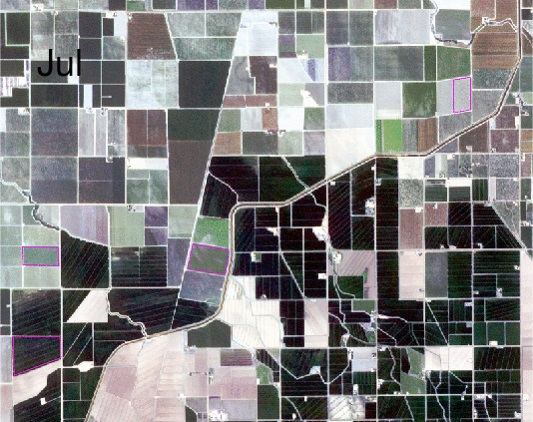
\includegraphics[width=1.0\textwidth]{Figures/testimage.jpg}
	\hspace{1mm}
	\caption{Test image include graphix.} 
	\label{fig:testimage}
\end{figure}

Snow is classified as wet or dry depending upon the amount of liquid water content. Dry snow consists of ice particles and air, whereas wet snow contains liquid water as a third component. Microwaves strongly respond to this change in liquid water content in snow~\citep{hallikainen1986dielectric}. The estimation of snowpack parameters requires a good understanding of the scattering mechanisms from the snowpack. Scattering from the air-snow surface and the uppermost layers are effective for wet snow estimation. The attenuation of a propagating EM wave is given in terms of the volume extinction coefficient ($\kappa_e$) and the penetration depth is defined as, $\delta_{p}=1/\kappa_e$. 



\section{Motivation}
\begin{itemize}
	\item SAR polarimetry is a very active research area in radar remote sensing in which there is an increased need to explore the potential for quantitative estimation of bio-/geo-physical parameters.
	
	\item Many works have reported the study of snow parameters using SAR data, among which very few studies barely attempted to retrieve any quantitative (for example snow wetness, snow density, snow grain size etc.) information.
	
	\item There is no proven precise methodology for the estimation of snowpack parameters using full polarimetric SAR data over the Indian Himalayan region. 
	
	\item The data obtained from the new generation advanced full-polarimetric SAR sensors along with the advanced polarimetric decomposition techniques, provide an opportunity to develop improved algorithms for snow pack parameters estimation. 
	
\end{itemize}
\section{Research objectives}
In this thesis, polarimetric SAR data is used for the estimation of snowpack parameters over the Indian Himalayan region. In this context algorithms have been developed for the estimation of snow wetness, snow surface dielectric constant and density,
\begin{description}
	\item[$\mbox{1(a)}.$ ] Estimation of snow wetness from dual polarimetric $(\mbox{HH}+\mbox{VV})$ coherent X-band data.
	\item[$\mbox{1(b)}.$ ] Estimation of snow wetness from full polarimetric $(\mbox{HH}+\mbox{HV}+\mbox{VH}+\mbox{VV})$ SAR data.
	\item[$\mbox{1(c)}.$ ] Estimation of snow surface dielectric constant from full polarimetric $(\mbox{HH}+\mbox{HV}+\mbox{VH}+\mbox{VV})$ SAR data.
	\item[$\mbox{2}.   $ ] Estimation of snow density from full polarimetric $(\mbox{HH}+\mbox{HV}+\mbox{VH}+\mbox{VV})$ C-band SAR data.
\end{description}

%\begin{enumerate}
%	
%\item Development of an algorithm for 
%	\begin{enumerate}
%	  \item Estimation of snow wetness from dual polarimetric $(\mbox{HH}+\mbox{VV})$ coherent TerraSAR-X X-band (9.65 GHz) data.
%	  \item Estimation of effective snowpack wetness from full polarimetric $(\mbox{HH}+\mbox{HV}+\mbox{VH}+\mbox{VV})$ Radarsat-2 (5.4 GHz) data.
%	  \item Estimation of snow surface dielectric constant from full polarimetric $(\mbox{HH}+\mbox{HV}+\mbox{VH}+\mbox{VV})$ SAR data.
%	\end{enumerate} 
%\item Development of an algorithm for estimation of snow density from full polarimetric $(\mbox{HH}+\mbox{HV}+\mbox{VH}+\mbox{VV})$ Radarsat-2 (5.4 GHz) data.
%\end{enumerate} 

These objectives are accomplished and implemented over the Indian Himalayan region for which data is acquired over the study area and field measurements were recorded during January to March 2012-2014. In the Indian Himalayan region, snowfall normally occurs during December to March from an altitude of 2000 m above the mean sea level. The expected snow wetness during Jan.-- Feb. is around 2--6 $\%$ by volume because of fresh snowfall and average minimum temperature. The snow density variation mainly depends on the temperature which produces the snow melt-freeze cycle. In the Indian Himalayan region, the mean minimum temperature in the month of January is around -15$^\circ$C-0$^\circ$C and the mean maximum temperature in the month of June is around 20$^\circ$C-30$^\circ$C. The mean high and low temperatures in the month of February over the study area are around 11$^\circ$C  and -1$^\circ$C respectively.
	  
\section{Thesis outline}
	The subject matter of the thesis is presented in the following five chapters, 
\begin{enumerate}[label=\checkmark]
\item	Chapter-1 gives an overview of the advantages of polarimetric SAR systems for snowpack parameters estimation. It also describes an outline of the snowpack parameters and their characteristics with respect to the electromagnetic waves, and also emphasizes the motivation of this research and objectives.
\item	Chapter-2 elucidates the principle and important parameters of a SAR system and the characteristics of snowpack parameters. Thorough investigations of snowpack characterization studies, PolSAR decomposition techniques and their advancements are included in this chapter. 
\item	Chapter 3 describes all the new developments of methodologies for the estimation of snow parameters from available SAR systems in separate subsections. All the new developments are presented with detailed flowcharts and derivations. The detailed description about the study area, in-situ field data collection and the data sets used for this study are incorporated in this chapter. 
\item Chapter-4 discusses the results obtained from all the algorithms and are presented in separate subsections along with detailed investigations using topographic and observatory measurements. Multi-temporal analyses of the results is also included in this chapter. 
\item	Chapter-5 highlights the new findings obtained by the utilization of SAR polarimetric data and conclusions arising out of this complete study are elucidated. The scope for future and continuation of this research work are also reported.  
%a new algorithm for the estimation of another important snowpack parameter, snow density is proposed using SAR polarimetry data. The detailed methodology with flow chart, snow density maps, thorough analysis of multi temporal variation of snow density within a season and the validation of the results are included in this section. 
%\item In Chapter-6, the proposed methodologies and the discussions of the results, including the important findings of the studies are summarized. The future scopes of the research works are proposed successively, following the conclusion on the basis of important extracts and understanding of the subject of interest.
\end{enumerate}


\chapter{Review of Literature}
\label{sec:2}
\section{Introduction}
In this Chapter, the emphasis of the discussion is on retrieval of snowpack parameters using spaceborne polarimetric SAR images. The principle and the imaging geometry of SAR system is described and a brief overview of the polarimetric SAR concepts are presented. A comprehensive exploration of all major factors affecting the SAR signal backscattered by the snow surface is discussed as available in the literature till date. 
\chapter{Development of Algorithms and Methodologies}
\label{sec:3}
In this chapter, all the new algorithms developed during the course of this work for the estimation of snow parameters from polarimetric SAR systems are explained. All the new methodologies are presented with detailed flowcharts and derivations. The detailed description about the study area, in-situ field data collection and the data sets used for this study are also incorporated in this chapter.


\chapter{Results and Discussions}
\label{sec:4}
In this Chapter, the results obtained from all the algorithms are presented in separate sub-sections along with the detailed investigations using topographic and observatory measurements. Multi-temporal analyses of the results are also presented. 
\section{Snow wetness from dual polarimetric data}
\FloatBarrier
In this section, the results obtained from the proposed snow wetness estimation method for dual-polarimetric coherent (HH/VV) SAR data (\emph{i.e.,} TerraSAR-X)~\cref{sec:3} are presented. 



\chapter{Summary and Conclusions}

In this thesis, the utilization of complete polarimetric SAR information for the estimation of snowpack parameters is described. Snow parameters in mountain areas are particularly sensitive to changes in environmental conditions. Timely gathering information about snow parameters and their temporal and spatial variability represents a significant contribution in climatology, local weather, avalanche forecasting and for the hydropower production in high mountainous areas. Conventional and ground-based methods represent only exact location measurements of field observations which may or may not be representative of a large area or basin. Due to the strong spatial and time-dependent dynamics of snow cover, frequent observation cycles are necessary. The sensitivity of microwave scattering to the characteristics of snowpack makes RADAR remote sensing a boon to understand a wide range of environmental issues related to the physical condition in high mountainous areas. Especially, the potential for retrieving snow parameters with a high spatial and/or temporal resolution corresponds to become an important input to snow avalanche forecasting, hydrological and meteorological modeling. 

Synthetic aperture radar (SAR) imaging technology is one of the most important advances in space-borne radar remote sensing during recent decades. In the present investigation, dual-~polarimetric (HH/VV) coherent TerraSAR-X (X-band) and full polarimetric Radarsat-2 (C-band) datasets have been used. Manali- Dhundhi region of Indian Himalaya is considered as a study area for this research work. Field data was collected synchronous with the satellite passes (Appendix-II). Snow parameters such as wetness, density, depth and snow permittivity have been measured using the snow fork instrument over the study area. Detailed analyses of  Microwave interaction with snow covered terrain and different scattering mechanisms are described in ~\cref{sec:2.3}, in order to understand the physical characteristics of snowpack parameters.

In this thesis, four major algorithms were presented for the estimation of snow wetness, snow surface dielectric constant and snow density. The algorithms have been proposed and validated using polarimetric SAR data and near real time in-situ measurements. The methodologies have been clearly explained in ~\cref{sec:3} comprising of four separate sections. The results obtained from these approaches have been meticulously presented with detailed discussions in ~\cref{sec:4} pertaining to the corresponding sections.

\begin{itemize}
	\item A new methodology for the estimation of snow wetness using dual-~polarimetric (HH/VV) coherent high frequency (9.6 GHz) SAR data has been proposed.  
	
	\item A new novel algorithm has been proposed to estimate snow wetness from full polarimetric SAR data. The proposed model was applied to Radarsat-2 fine resolution full-polarimetric data sets acquired over the Indian Himalayan region for three consecutive years.   
	
	\item Snow surface dielectric constant estimation methodology from full-polarimetric SAR data is proposed. The dominant scattering type amplitude ($\alpha_{s1}$) is used to characterize dominant snow.
	
	\item At final, a new methodology for snow density estimation from C-band full--polarimetric SAR data is proposed. The generalized volume parameter is derived from the double unitary transformation of the coherency matrix. 
	
	\item These research works have been assimilated in the HimSAR software toolbox which is under development and expansion for the cryospheric applications using polarimetric SAR data. This toolbox will be helpful for the cryospheric scientific community to utilize, explore and contribute to the further development of this open source toolbox.
	   
\end{itemize}
\section{Contributions}
During this course of research work, four major contributions were made in-terms of new algorithms development for the estimation of snowpack parameters. 
\begin{itemize}
	\item A new snow wetness estimation algorithm is developed for dual.  
	\item A new novel algorithm has been developed to estimate snow wetness using full polarimetric SAR data.  
	\item Snow surface dielectric constant estimation methodology has been developed for full-polarimetric SAR data.   
	\item A new methodology for snow density estimation from C-band full--polarimetric SAR data is developed.  
\end{itemize}
\section{Scope for future research}
\begin{itemize}
	\item The proposed snowpack parameters estimation algorithm can be extended for multi frequency SAR data by considering all possible scattering mechanisms.
	\item Particularly for the estimation of snow density where the snowpack volume scattering has only been considered for the Radarsat-2 C-band data.  
\end{itemize}
  




 




%=====================================================================
% APPENDIX
%  Appendices, if any, must precede the cited literatures.
%  Appendices shall be numbered in Roman Capitals (e.g. Appendix IV)


\begin{appendices}
	\chapter{Measurement system}

\section{Introduction}
Here we go... decomposition methodologies available in the literature. Moreover, it also contains algorithms for snowpack parameters estimation from single, dual and full- polarimetric SAR data. 

\section{Functionalities}
Many pre and post-processing steps are included along with the snowpack parameter estimation algorithms in this HimSAR toolbox.
	\chapter{Measurements Techniques}
Field campaigns were conducted in month of February over the study area. 





\end{appendices}


 
        

%=====================================================================
% BIBLIOGRAPHY
\newpage
\setlength{\parskip}{5mm}
\titlespacing{\chapter}{0cm}{0mm}{0mm}
\titleformat{\chapter}[display]
  {\normalfont\huge\bfseries}
  {\chaptertitlename\ \thechapter}{20pt}{\Huge}


\bibliographystyle{References/elsarticle-harv}
% Add the bib file
\bibliography{References/mybibfile}

%=====================================================================
% PUBLICATIONS
%  publications if any may be listed after the literature cited.
%\addcontentsline{toc}{chapter}{List of Publications}
\chapter*{List of Publications}
\label{ch:pub}
\addcontentsline{toc}{chapter}{\nameref{ch:pub}}

%\section*{Book Chapter}
%\begin{enumerate}
% \item \textbf{S. K. Panda}, S. S. Gedam, and S. jin, 2015, \textquotedblleft Ionospheric TEC variations at low latitude Indian region\textquotedblright, \textit{In Book Satellite Positioning: Methods, Models and Applications}, InTech-Publisher, Rijeka, Croatia. (Accepted, In Press).
%\end{enumerate}
   
\section*{International Journals}
\begin{enumerate}
	
	\item Bhattacharya. A, \textbf{Surendar. M}, 2016,\textquotedblleft Enhanced Target Detection and Improved Scattering Power Decompositions Using the Optimized Coherency Matrix from Full-Polarimetric SAR Data \textquotedblright, \textit{Geoscience and Remote Sensing Letters, IEEE}, (Under revision)
	
	\item \textbf{Surendar. M}, Bhattacharya. A, Singh. G,  Yamaguchi. Y, 2016,\textquotedblleft Estimation of snow surface dielectric constant from polarimetric SAR data \textquotedblright, \textit{Journal of Selected Topics in Applied Earth Observations and Remote Sensing, IEEE}, (Under revision)
	
	\item Pandey. P, \textbf{Surendar. M}, Bhattacharya. A, Ramanathan. A.L, Singh. G, Venkataraman. G, 2015,\textquotedblleft Qualitative and quantitative assessment of TanDEM-X DEM over western Himalayan glaciated terrain \textquotedblright, \textit{Geocarto International}, (In Press)
	
	
\end{enumerate}
\section*{International Conferences}
  \begin{enumerate}
  \item Banerjee, B, De. S, \textbf{Surendar. M}, Bhattacharya, A, 2016 \textquotedblleft An Unsupervised hidden markov random field based segmentation of polarimetric SAR images\textquotedblright, \textit{Geoscience and Remote Sensing Symposium (IGARSS), IEEE International}, (submitted)
  
  \item Deo. R, \textbf{Surendar. M}, Rao. Y.S, Gedam. S.S, 2013 \textquotedblleft Evaluation of interferometric SAR DEMs generated using TanDEM-X data\textquotedblright, \textit{Geoscience and Remote Sensing Symposium (IGARSS), IEEE International}, pp.2079-2082, 21-26 July 2013 \break doi:10.1109/IGARSS.2013.6723221.

\item \textbf{Surendar. M}, Bhattacharya. A, Singh. G, Venkataraman. G, Bharathi, P.A, 2013 \textquotedblleft Snow wetness estimation from polarimetric SAR image\textquotedblright, \textit{Progress In Electromagnetics Research Symposium (PIERS)}, Stockholm, Sweden, Aug. 12-15, 2013, pp.678-682.

\item \textbf{Surendar. M}, Bhattacharya. A, Venkataraman. G, 2013 \textquotedblleft Glacier Velocity Estimation Using Offset Tracking Method\textquotedblright, \textit{TerraSAR-X/TanDEM-X Science Team Meeting}, DLR, 2013, Oberpfaffenhofen, Germany, https://tandemx-science.dlr.de/pdfs.



\end{enumerate}
%\section*{National Conferences}
%  \begin{enumerate}
%  \item \textbf{S. K. Panda}, S. S. Gedam, and G. Rajaram, 2014, \textquotedblleft Investigations of Geomagnetic storm effect on the equatorial ionospheric anomaly over Indian region with GPS, Radio occultation and magnetometer observations\textquotedblright, \textit{Proc. of  National Conference on Application of  Geoinformatics in Rural, Urban \& Climatic Studies (Geomatrix’14)}, Indian Institute of Technology Bombay, CD proceedings.
%  \item \textbf{S. K. Panda} and S. S. Gedam, 2012, \textquotedblleft Investigating ionospheric total electron content over low latitude Indian region by analysis of GPS signals during ascending part of 24th Solar cycle\textquotedblright, \textit{National Symposium on ‘Space Technology for Food \& Environmental Security’ \& Annual Convention of Indian Society of Remote Sensing \& Indian Society of Geomatics}, Delhi, India, Abstract proceedings.
%\end{enumerate}

%=====================================================================
% ACKNOWLEDGMENTS
%   This is the last item in the thesis. It should be signed by
%   author, with date.


\newpage
\setlength{\parskip}{5mm}
\titlespacing{\chapter}{0cm}{0mm}{0mm}
\titleformat{\chapter}[display]
  {\normalfont\huge\bfseries \centering}
  {\chaptertitlename\ \thechapter}{20pt}{\Huge}

\chapter*{Acknowledgments}
\label{ch:Acknowledgments}
\addcontentsline{toc}{chapter}{\nameref{ch:Acknowledgments}}
\vspace{10mm}
I wish to record a deep sense of gratitude to \textbf{Prof. ..}, my supervisor for his valuable guidance and constant support at all stages of my Ph.D study and related research. 


\end{document}
